\documentclass[stu, floatsintext]{apa7}

\usepackage[american]{babel}
\usepackage{csquotes}
\usepackage[style=apa, backend=biber]{biblatex}
\addbibresource{references.bib}

\usepackage{booktabs}
\usepackage{threeparttable}
\usepackage{array}
\usepackage{graphicx}

\title{Composer Classification from Symbolic MIDI: LSTM and CNN Baselines on a Fixed File-Level Split}
\shorttitle{Composer Classification with Deep Learning}

\authorsnames{Marston Ward, Josue Sandoval, and Saman Tavasoli}
\authorsaffiliations{University of San Diego}

\course{AAI-511: Neural Networks and Deep Learning}
\professor{Professor Andrew Van Benschoten}
\duedate{\today}

\abstract{This paper compares deep learning baselines for attributing classical
  MIDI files to Bach, Beethoven, Chopin, or Mozart. After unreadable files and
  exact byte duplicates were removed, individual MIDI files were assigned to a
  fixed, stratified train, validation, and test manifest; movements from the same
  work were not grouped. PyTorch long short-term memory (LSTM) and
  one-dimensional convolutional neural network (CNN) models consume fixed-length
  sequences of pitch, velocity, note duration, and onset interval. Class-weighted
  loss addresses training-set imbalance, while weight decay and validation-based
  early stopping constrain model fitting. At their selected checkpoints in one
  seeded MPS run, the CNN achieved .822 validation accuracy and .812 weighted F1,
  compared with .759 accuracy and .748 weighted F1 for the LSTM. Local pattern
  detection is one plausible explanation for the CNN's advantage, but a single
  run without architecture ablations cannot identify the cause. The CNN's .982
  training accuracy and .822 validation accuracy also show substantial
  overfitting on this split. The CNN is therefore the stronger baseline on this
  file-level validation split, but cross-partition works, nondeterministic
  training, and the held-out test set preclude claims of stable or unseen-work
  generalization. The highest-priority improvements are work-grouped data
  partitions, repeated deterministic runs, and controlled architecture and
  regularization ablations before one final test-set evaluation.}

\keywords{composer classification, MIDI, deep learning, LSTM, CNN, music information retrieval}

\begin{document}
\maketitle

Automatic composer identification is a long-standing music information retrieval
problem: given a piece of music, predict which composer wrote it. Symbolic
representations such as MIDI expose pitch, duration, and timing information
directly, without the confounds of audio timbre or recording conditions, making
them a natural substrate for sequence and pattern-based deep learning models.

\section{Related Work}
\textcite{Hochreiter1997} introduced the long short-term memory architecture,
which remains a standard approach for modeling long-range dependencies in
sequential data such as musical note sequences. \textcite{LeCun2015} describe
convolutional architectures that motivate the CNN comparison using a
structured music representation. \textcite{Kingma2015} introduced the Adam
optimizer used to train both baselines.

Symbolic-music classification commonly combines engineered representations with
statistical or machine-learning models. \textcite{Conklin2013} demonstrated how
multiple musical viewpoints can support classification, while
\textcite{McKay2018} presented jSymbolic, a reproducible framework for extracting
features from symbolic music. The present comparison instead learns directly
from fixed-length note sequences while retaining aggregate features for EDA.

\section{Method}

\subsection{Dataset}
The dataset used for this project is the \textit{MIDI Classic Music} corpus from
Kaggle \parencite{FedorakND}. Kaggle identifies the archive as Version 1 and
lists its license as unknown. The archive contains MIDI files for many
classical composers; for this study we filtered it to the four required
composers: Bach, Beethoven, Chopin, and Mozart. The helper script
\texttt{src/prepare\_dataset.py} downloads the archive (when
\texttt{{\raise.17ex\hbox{$\scriptstyle\sim$}}/.kaggle/kaggle.json} is
configured), extracts the four composer folders, and creates
filtered copies for optional inspection. The modeling workflow does not use
those copied splits. Instead, \texttt{src/data\_pipeline.py} scans the four raw
composer folders, excludes unreadable files and exact duplicates, and creates
the controlling stratified 70/15/15 file-level train, validation, and test
manifest with a fixed random seed. The manifest is reused unless regeneration is
explicitly requested, preventing accidental resampling between experiments.
Files are not grouped by musical work, catalog number, or source collection;
for example, movements of Mozart's Symphony No. 40, K. 550 occur in all three
partitions. Consequently, the validation results measure performance on held-out
files from this corpus and may be optimistic for unseen works. Class balance
across the cleaned corpus is reported in the accompanying master notebook.

The cleaned corpus contains 1,608 MIDI files: 1,125 training, 241 validation,
and 242 test files. Twenty-two files were excluded as malformed or exact
duplicates. Bach accounts for roughly 63\% of the training files (709 of
1,125), whereas Chopin contributes 8\% (92 of 1,125). To reduce majority-class
bias, both models use class-weighted cross-entropy loss. We report validation
accuracy, per-class precision, recall, F1 scores, and a confusion matrix; the
test split is not used during baseline development.

\subsection{Computational Workflow}
The repository uses Pixi to create a project-local, locked Python 3.12
environment, and the saved manifest fixes file assignments. After
\texttt{pixi install}, collaborators run \texttt{pixi run
prepare-dataset} to obtain the raw corpus and \texttt{pixi run notebook} to
launch the master notebook. The environment selects Apple Metal Performance
Shaders (MPS) when available, then CUDA, and finally CPU. These controls make the
software environment and preprocessing repeatable, but exact training metrics
are not guaranteed across runs or devices because deterministic PyTorch
algorithms are not enforced and device-specific batch sizes differ. The master
notebook is an orchestration and reporting document: reusable data preparation,
feature extraction, model, training, and visualization logic resides in
\texttt{src/}.

MIDI-level EDA metadata are saved to
\texttt{dataset/processed/eda\_metadata.csv} after the initial parse. Subsequent
runs load this cache unless an explicit refresh is requested. Thus, the notebook
presents the same training-split EDA tables and plots without reparsing every
MIDI file on each model run. Because the cache is not automatically validated
against the manifest, it must be refreshed after intentional data or manifest
changes.

\subsection{Exploratory Data Analysis}
Before modeling, metadata are extracted for the clean manifest: duration, tempo,
note count, note density, pitch range, and mean pitch. The cached metadata are
summarized only on the training split, protecting validation and test files from
informing exploratory decisions. Table~\ref{tab:eda-summary} summarizes these
features by composer.

\begin{table}[htbp]
  \centering
  \begin{threeparttable}
    \caption{Composer-Level Feature Summary (Train Split)}
    \label{tab:eda-summary}
    \begin{tabular}{@{}lrrrr@{}}
      \toprule
      Composer & \shortstack{Duration\\(s)} & \shortstack{Note density\\(notes/s)} & \shortstack{Pitch range\\(semitones)} & \shortstack{Tempo\\(BPM)} \\
      \midrule
      Bach      & 160.3 & 9.3  & 43.1 & 89.7  \\
      Beethoven & 518.3 & 14.5 & 61.1 & 123.3 \\
      Chopin    & 222.3 & 11.6 & 63.0 & 112.0 \\
      Mozart    & 415.5 & 13.7 & 55.3 & 104.9 \\
      \bottomrule
    \end{tabular}
    \tablenote{Values are per-composer means computed from cached, parsed MIDI
      metadata. Unreadable files and exact duplicates are excluded by the clean
      manifest.}
  \end{threeparttable}
\end{table}

Three descriptive patterns informed feature selection. First, mean note density
differs across composers---Bach averages 9.3 notes/s while Beethoven averages
14.5 notes/s---whereas raw note count is correlated with file duration. Second,
mean pitch range is lower for Bach ($M = 43.1$ semitones) than for Beethoven and
Chopin ($M \approx 62$ semitones). These corpus-level differences may also
reflect instrumentation, arrangement, source, or MIDI-encoding conventions and
do not establish causal stylistic or historical explanations. Third, tempo and
note velocity can reflect encoding defaults rather than performed values, so
they are interpreted cautiously.

A principal component analysis of the engineered statistical features showed
substantial class overlap in its first two components. This limited visual
separation motivated testing sequence representations that preserve temporal and
structural information, but it does not establish that all summary-feature
classifiers would fail: the plot omits 34.4\% of standardized variance, and no
engineered-feature classifier was evaluated.

Quantitatively, the first principal component explained 47.1\% of variance and
the second explained 18.5\% (65.6\% cumulative), yet the composer classes still
overlap heavily in two dimensions. Correlation analysis found that raw note
count and duration are coupled ($r = .69$), so we prioritize derived features
such as note density and temporal representations that preserve rhythmic
structure rather than relying only on aggregate counts. Both analyses are
computed by the canonical master workflow from training rows only and are shown
in Figure~\ref{fig:eda-analysis}.

\begin{figure}[htbp]
  \centering
  \caption{Training-split PCA scores (left) and EDA feature correlations (right).}
  \label{fig:eda-analysis}
  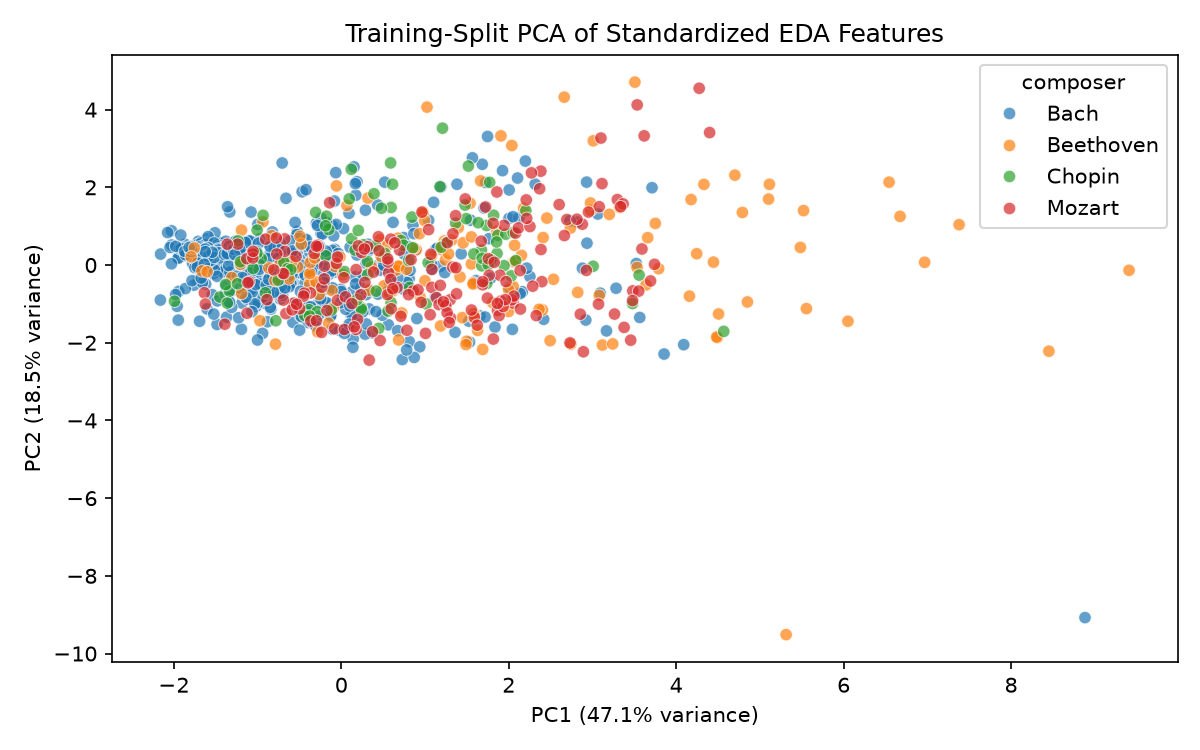
\includegraphics[width=.48\textwidth]{../figures/eda_pca.png}
  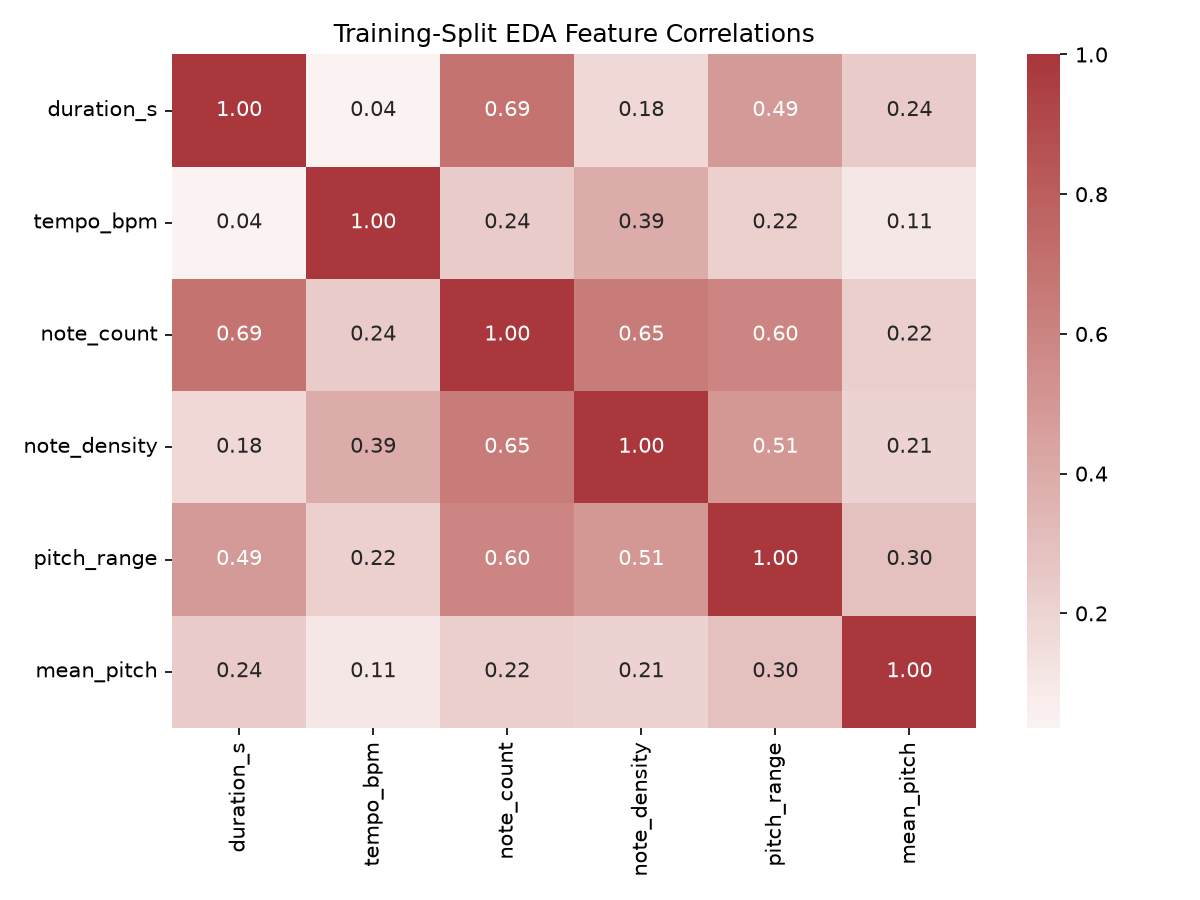
\includegraphics[width=.48\textwidth]{../figures/eda_correlation.png}
\end{figure}

\subsection{Preprocessing and Feature Extraction}
For both model inputs, notes are ordered by onset, pitch, and end time. Each note is
represented by four values: a pitch token in $[1,128]$, MIDI velocity, duration,
and elapsed time since the preceding onset. A zero token marks padded positions.
Sequences are truncated or padded to 4,096 notes. Velocity, duration, and onset
interval are normalized with statistics estimated from nonpadding notes in the
training split only; those same statistics are then applied to validation and
test data. This prevents leakage from validation or test distributions into the
feature transformation.

\subsection{Model Architectures}

\subsubsection{LSTM Model}
The implemented baseline embeds the pitch token into 32 dimensions, concatenates
the embedding with the three normalized continuous features, and passes the
result through a one-layer LSTM with 64 hidden units. Dropout ($p = .30$) is
applied to the final state before a four-unit linear classifier. The final state
corresponding to the last nonpadding note is used for prediction, so padding does
not determine the piece representation.

\subsubsection{CNN Model}
The implemented one-dimensional CNN uses the same 32-dimensional pitch embedding
and three normalized continuous features as the LSTM. The concatenated
35-channel note representation passes through convolutional blocks with 64,
128, and 128 filters. The first two blocks use kernels of width five and
four-note max pooling; the third uses a kernel of width three. Batch
normalization and ReLU follow each convolution. Adaptive global max pooling
creates a piece-level representation, which passes through dropout ($p = .30$)
and a four-unit linear classifier. The CNN uses the same clean manifest, split
assignments, training-only normalization, class-weighting strategy, and
validation-based model selection as the LSTM.

\subsection{Training}
Both baselines are trained for up to 20 epochs with Adam \parencite{Kingma2015}
at a learning rate of .001 and a weight decay of $1\times10^{-4}$. Inverse-frequency
class weights are computed from the training labels as $w_c = N/(K n_c)$, where
$N$ is the number of training files, $K$ is the number of classes, and $n_c$ is
the number of files for class $c$. Gradients are clipped to a maximum norm of
1.0. At every epoch, the model is evaluated on the validation split. The
checkpoint with the highest validation accuracy is retained; validation loss
breaks ties. Training stops early once five consecutive epochs pass without a
new best checkpoint. In the reported weight-decayed run, CNN training accuracy
reached 96.8\% at epoch 20 while validation loss was unstable, and the LSTM's
validation loss began rising after epoch 10 despite falling training loss. These
patterns show that the configured regularization did not eliminate overfitting;
no preserved ablation isolates the effects of weight decay or early stopping.
Neither augmentation nor a test result is claimed because the test split remains
held out.

\section{Results}
The master notebook evaluated both baselines on the same 241-file validation
split. In this seeded MPS run, the CNN was the stronger validation model,
improving accuracy by 6.2 percentage points and weighted F1 by 6.4 percentage
points over the LSTM. Table~\ref{tab:results} reports the selected checkpoints.
The 242-file test split remains sealed.

\begin{table}[htbp]
  \centering
  \begin{threeparttable}
    \caption{Validation Results for Selected Baselines}
    \label{tab:results}
    \begin{tabular}{@{}lrrrrl@{}}
      \toprule
      Model & Epoch & Accuracy & \shortstack{Weighted\\F1} & \shortstack{Macro\\F1} & Test evaluation \\
      \midrule
      LSTM baseline & 6 & .759 & .748 & .622 & Reserved \\
      CNN baseline & 18 & .822 & .812 & .710 & Reserved \\
      \bottomrule
    \end{tabular}
    \tablenote{Metrics are from validation-selected checkpoints trained with
      weight-decayed Adam on the fixed clean manifest. The test split was not
      evaluated.}
  \end{threeparttable}
\end{table}

Figure~\ref{fig:loss-curves} shows that the LSTM triggered early stopping at
epoch 11, while the CNN reached the 20-epoch budget and retained its epoch-18
checkpoint. A separate evaluation of that restored CNN checkpoint measured
98.2\% training accuracy and 82.2\% validation accuracy, confirming that
substantial overfitting remains. Figure~\ref{fig:validation-matrices} shows the
class-level outcome. The CNN improved recall for Chopin (.800 versus .650) and
Beethoven (.613 versus .258), while both models continued to underperform on
Beethoven and Mozart relative to Bach.

\begin{figure}[htbp]
  \centering
  \caption{Training and validation loss for the LSTM (left) and CNN (right).}
  \label{fig:loss-curves}
  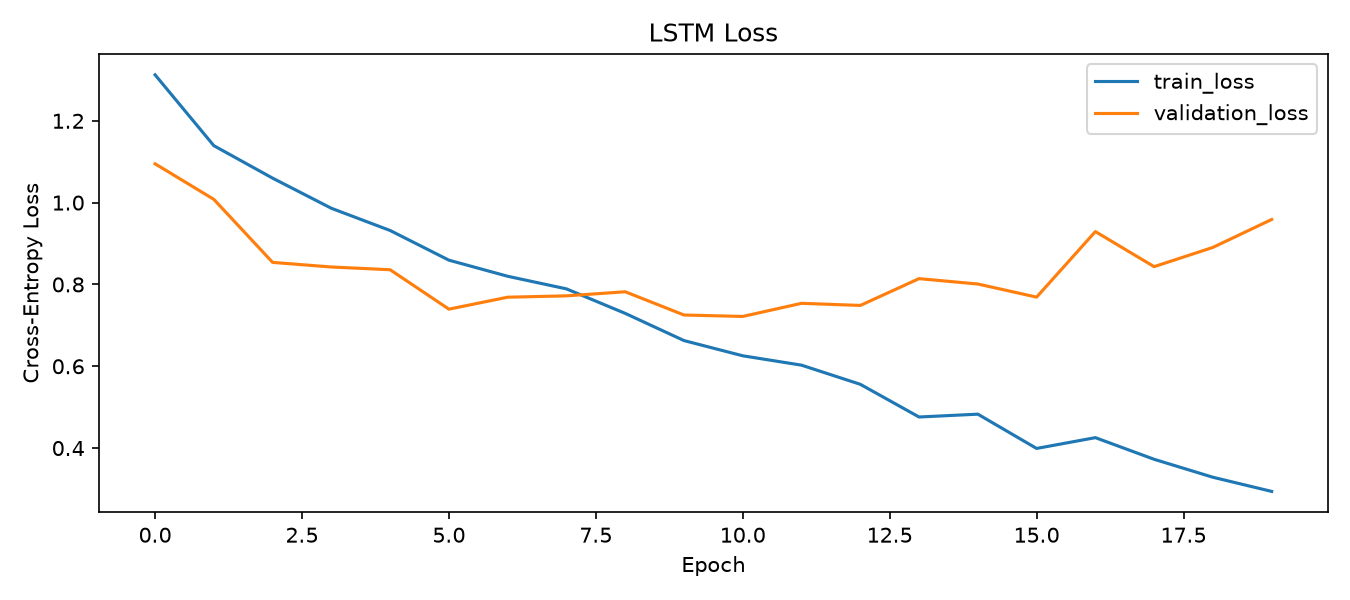
\includegraphics[width=.48\textwidth]{../figures/lstm_loss.png}
  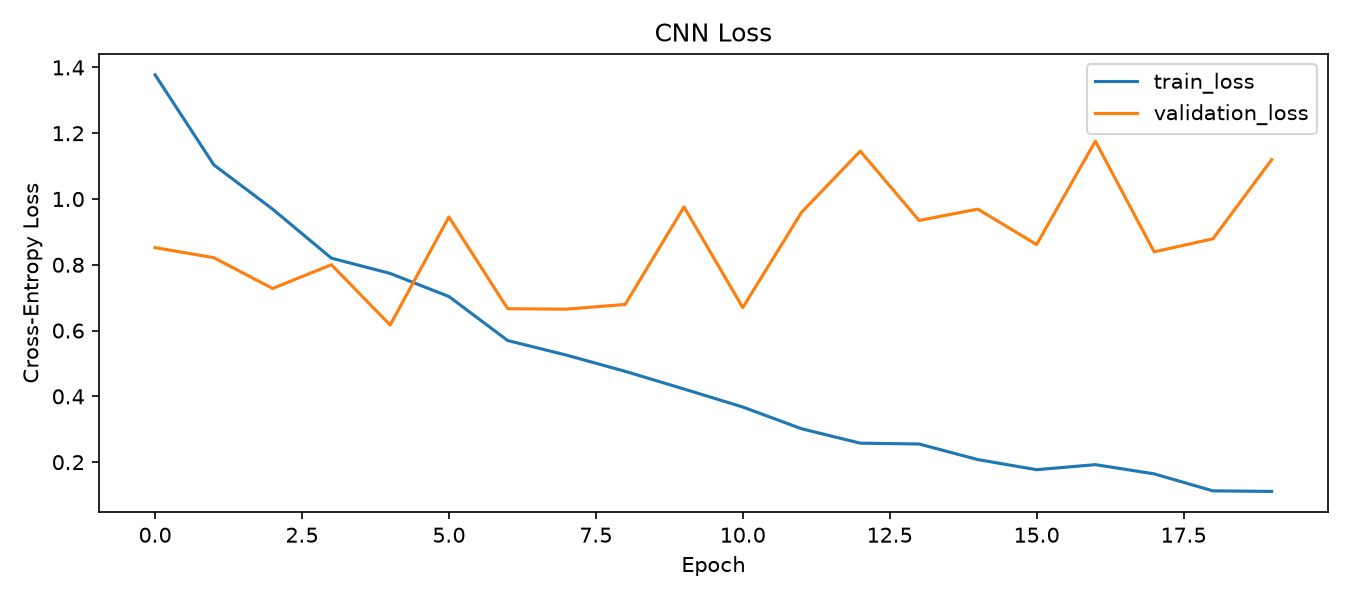
\includegraphics[width=.48\textwidth]{../figures/cnn_loss.png}
\end{figure}

\begin{figure}[htbp]
  \centering
  \caption{Validation confusion matrices for the LSTM (left) and CNN (right).}
  \label{fig:validation-matrices}
  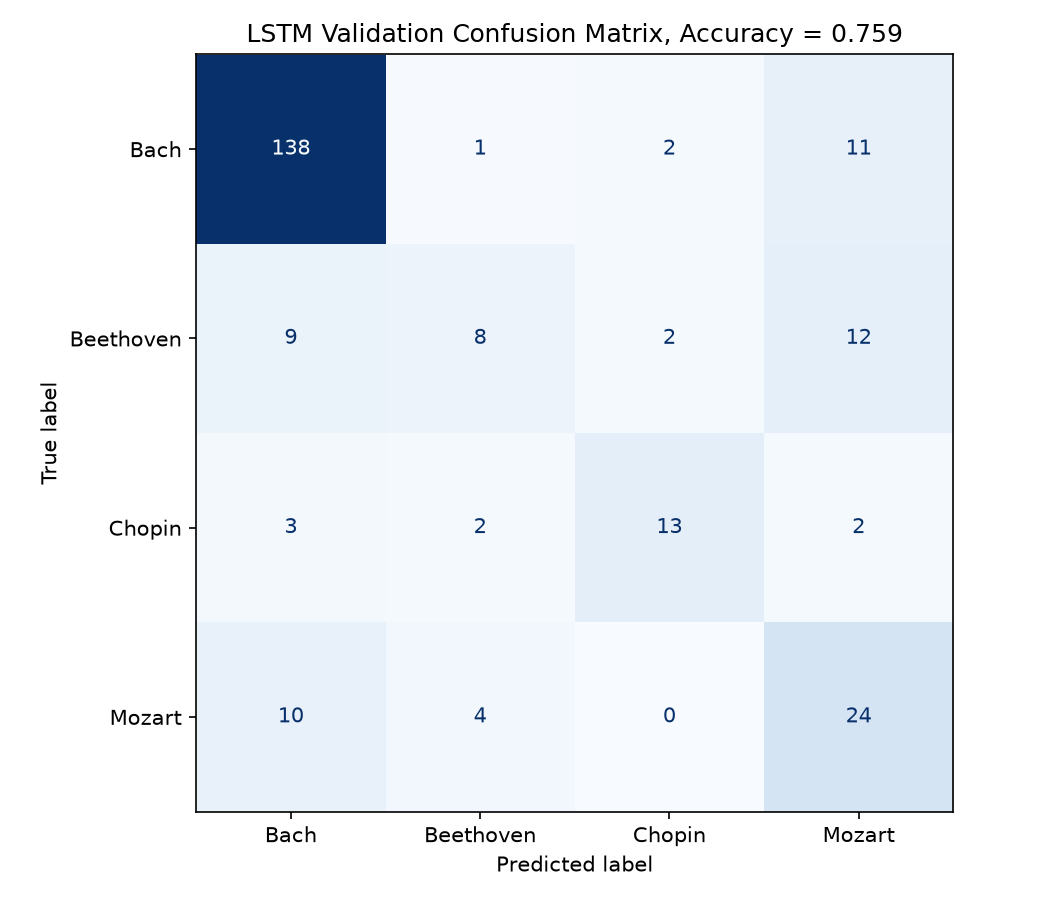
\includegraphics[width=.48\textwidth]{../figures/lstm_validation_confusion_matrix.png}
  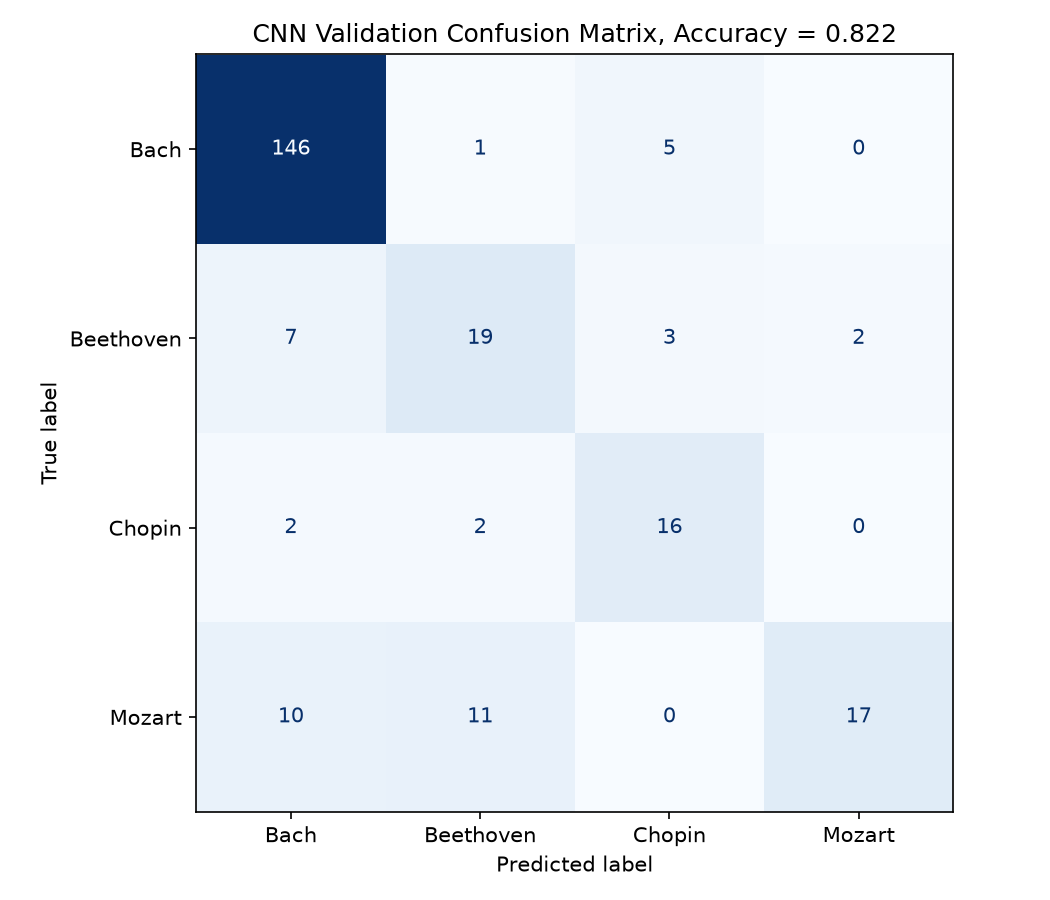
\includegraphics[width=.48\textwidth]{../figures/cnn_validation_confusion_matrix.png}
\end{figure}

\section{Discussion}
The validation comparison favors the CNN, but it is not a final generalization
claim because the test split remains unused. The LSTM models sequence order,
while the CNN preserves local ordered patterns before position-invariant global
max pooling; both consume duration, velocity, and local timing information that
the aggregate EDA summaries discard. Class weighting was applied because Bach
dominates the training set; an unweighted ablation would be required to quantify
its effect. The class-specific reports show that accuracy alone conceals lower
recall for Beethoven and Mozart.

Weight decay and validation-based early stopping were applied to both models,
but no preserved unregularized ablation supports a causal claim about how much
either intervention improved generalization. The selected CNN checkpoint still
exhibits about a 16-point train--validation accuracy gap. Validation-based
checkpoint selection introduces within-run selection optimism; the held-out test
evaluation is needed for the final estimate.

The CNN's stacked local filters and global max pooling offer one plausible
explanation for its higher score, but this interpretation is post hoc. The CNN
also differs from the LSTM in capacity, batch normalization, pooling, and
padding treatment. Repeated seeds and controlled ablations would be required to
attribute the observed difference to local-pattern detection.

The workflow establishes a fair comparison condition: both architectures use the
same fixed manifest, feature transformation, class weighting, and test-isolation
policy. Their final hyperparameters should be selected only from validation
performance, then both final models should be evaluated once on the held-out test
split. Because related movements and collections can occur across partitions,
even that test would estimate file-level performance on this corpus rather than
generalization to unseen works. The reported comparison is also one seeded
accelerator run and should be interpreted descriptively rather than as evidence
of stable architectural superiority; repeated seeds would be required to
quantify run-to-run variance.

\section{Conclusion}
This project establishes a fixed file-level symbolic-MIDI
composer-classification pipeline and implements LSTM and CNN baselines. Pixi
locks the software environment, the manifest fixes file assignments, and the
master notebook presents results from reusable version-controlled modules. Under
the shared validation protocol, the CNN achieved the higher score in this run,
but its train--validation gap shows that substantial overfitting remains. The
evidence therefore identifies the CNN as the stronger baseline for this
file-level split, not as a generally superior architecture. Claims about stable
or unseen-work generalization require grouped work-level splits, repeated seeds,
and a single final evaluation of models selected without test-set feedback.

The first improvement should be to assign a work or collection identifier before
splitting so that related movements cannot cross partitions. Evaluation should
then use repeated seeds with deterministic PyTorch settings, a fixed batch size
across devices, and mean performance with run-to-run variation rather than one
accelerator run. Controlled ablations should isolate the effects of class
weighting, weight decay, early stopping, model capacity, and the CNN's pooling
strategy; masking padded positions before global pooling would also remove
sequence-length artifacts as a possible explanation for its advantage. If
overfitting persists, stronger dropout, a smaller CNN, and musically valid pitch,
tempo, or timing augmentation should be compared using validation data only.
After those choices are fixed, the held-out test split should be evaluated once;
a work-grouped test split would provide the most defensible estimate of
generalization to previously unseen compositions.

\printbibliography

\end{document}
